\documentclass[a4paper,fleqn]{cas-sc}

\usepackage[numbers,sort&compress]{natbib}
\usepackage{amsmath,amsfonts,amssymb,amsthm}
\usepackage{booktabs}
\usepackage{multirow}
\usepackage{graphicx}
\usepackage{hyperref}
\usepackage{microtype}
\usepackage{listings}
\usepackage{xcolor}

% Cấu hình hỗ trợ tiếng Việt đa nền tảng
\usepackage{iftex}
\ifPDFTeX
  \usepackage[utf8]{inputenc}
  \usepackage[vietnamese,english]{babel}
  \usepackage[T5,T1]{fontenc}
\else
  \usepackage{fontspec}
  \usepackage[vietnamese,english]{babel}
\fi

\newtheorem{definition}{Định nghĩa}
\newtheorem{theorem}{Định lý}
\newtheorem{lemma}{Bổ đề}
\newtheorem{proposition}{Mệnh đề}

\begin{document}
\selectlanguage{vietnamese}

\let\WriteBookmarks\relax
\def\floatpagepagefraction{1}
\def\textpagefraction{.001}

% Header tiêu đề và tác giả
\shorttitle{Nghiên cứu các Kỹ thuật Mã hóa SAT cho Bài toán N-Queens}
\shortauthors{Nguyễn Văn A}

% Tiêu đề chính
\title [mode = title]{Nghiên cứu các Kỹ thuật Mã hóa SAT cho Bài toán N-Queens và So sánh Thực nghiệm với Quy hoạch Tuyến tính Nguyên (ILP) và Lập trình Ràng buộc (CP)}

% Thông tin tác giả (Sinh viên cập nhật thông tin chính xác tại đây)
% Ghi chú: Ký hiệu [1] trong \author[1] là nhãn tham chiếu đơn vị công tác (\address[1]), hiển thị dạng chỉ số trên trong PDF.
\author[1]{Nguyễn Văn A}[role=Sinh viên thực hiện]
\cormark[1]
\ead{24020000@vnu.edu.vn}

\author[1]{TS. Tô Văn Khánh}[role=Giảng viên hướng dẫn]
\ead{khanhtv@vnu.edu.vn}

\address[1]{Khoa Công nghệ Thông tin, Trường Đại học Công nghệ, Đại học Quốc gia Hà Nội, 144 Xuân Thủy, Cầu Giấy, Hà Nội, Việt Nam}

\cortext[cor1]{Tác giả liên hệ chính (Mã số sinh viên: 24020000).}

\begin{abstract}
Bài toán $N$-Queens là bài toán kinh điển trong khoa học máy tính và tối ưu tổ hợp rời rạc, yêu cầu sắp xếp $N$ quân hậu trên bàn cờ $N \times N$ sao cho không có hai quân hậu nào cùng hàng, cùng cột hoặc cùng đường chéo. Khi kích thước $N$ gia tăng, không gian tìm kiếm bùng nổ theo giai thừa $\mathcal{O}(N!)$, đặt ra thử thách lớn đối với các bộ giải chính xác. Trong bài báo này, chúng tôi nghiên cứu và triển khai tiếp cận giải chính xác bài toán $N$-Queens bằng phương pháp SAT Solving thông qua thư viện PySAT. Trọng tâm của bài báo là khảo sát, so sánh lý thuyết và đánh giá định lượng 5 kỹ thuật mã hóa ràng buộc At-Most-One (AMO): Pairwise (Direct), Sequential Counter (Sinz, 2005), Commander Variable (Klieber \& Kwon, 2007), Binary (Frisch et al., 2005; Prestwich, 2009) và Product Encoding (Chen, 2010). Chúng tôi phân định rõ ràng giữa các phương pháp gọi qua bộ mã hóa tích hợp của PySAT và các phương pháp tự cài đặt theo bài báo gốc. Kết quả phân tích và thực nghiệm cho thấy mã hóa Pairwise bùng nổ đa thức bậc ba $\mathcal{O}(N^3)$ mệnh đề trên toàn bàn cờ, dẫn tới tiêu tốn khoảng 4 GB RAM đỉnh tại $N=256$ ($4{,}073.8$ MB, tương đương $\approx 3.98$ GiB) và cạn kiệt bộ nhớ (Out-Of-Memory) khi tạo $207{,}834{,}500$ mệnh đề (xấp xỉ $207.8$ triệu) trong cấu trúc danh sách Python tại $N=500$; trong khi Sequential Counter, Product và Commander duy trì bậc $\mathcal{O}(N^2)$ mệnh đề toàn cục. Về hiệu năng giải bằng CaDiCaL 1.9.5, Commander Variable cho tốc độ nhanh nhất ở dải $N \in [16, 128]$ (chỉ mất $0.62$s ở $N=128$). Ở quy mô cực đại $N \ge 256$, cả Commander Variable và Product Encoding đều thể hiện năng lực mở rộng vượt bậc, giải quyết thành công $N=500$ (Commander: $35.22$s, Product: $36.02$s) và $N=1000$ ($1{,}000{,}000$ ô cờ; Commander: $138.15$s, Product: $263.82$s) với thời gian giải tương đương nhau và có sự dao động giữa các lần chạy do đặc thù tìm kiếm của thuật toán CDCL. Đồng thời, chúng tôi tiến hành so sánh đối chứng nghiêm ngặt (chạy đơn luồng, cùng Time Limit 300.0s cho thời gian giải, lấy trung vị 3 lần lặp độc lập trong các tiến trình riêng biệt cho mọi $N$) với các bộ giải CP-SAT (Google OR-Tools), Gurobi Optimizer 13.0 và SCIP 9.0 (ILP MIP). Kết quả cho thấy SAT Solving thể hiện ưu thế vượt trội về khả năng mở rộng ở các kích thước $N \ge 256$ so với SCIP và CP-SAT, trong khi Gurobi thể hiện tốc độ nhanh nhất ở quy mô nhỏ ($N \le 32$) nhưng dừng ở $N \ge 64$ do giới hạn kích thước bản quyền học thuật thử nghiệm (2,000 biến).
\end{abstract}

\begin{keywords}
$N$-Queens \sep SAT Solving \sep PySAT \sep CaDiCaL \sep At-Most-One (AMO) \sep Commander Variable \sep Product Encoding \sep Constraint Programming (CP) \sep Integer Linear Programming (ILP) \sep Gurobi
\end{keywords}

\maketitle

\section{Giới thiệu (Introduction)}
Bài toán $N$-Queens (xếp $N$ quân hậu) được nhà nghiên cứu Max Bezzel khởi xướng vào năm 1848 dưới dạng bài toán 8 quân hậu trên bàn cờ vua tiêu chuẩn, và nhanh chóng thu hút sự chú ý của các nhà toán học lừng danh, tiêu biểu là Carl Friedrich Gauss~\cite{bell2009survey}. Về mặt hình thức, bài toán yêu cầu đặt $N$ quân hậu lên một bàn cờ kích thước $N \times N$ sao cho không có bất kỳ hai quân hậu nào có thể tấn công lẫn nhau. Theo luật cờ vua, điều này đồng nghĩa với việc không có hai quân hậu nào nằm trên cùng một hàng, cùng một cột, hoặc cùng một đường chéo (chính hoặc phụ).

Mặc dù có cấu trúc phát biểu trực quan và đơn giản, $N$-Queens là bài toán chuẩn mực (standard benchmark) để kiểm tra năng lực của các thuật toán tìm kiếm tổ hợp, kỹ thuật thỏa mãn ràng buộc (CSP - Constraint Satisfaction Problem), giải thuật heuristic và các bộ giải suy diễn logic~\cite{rossi2006handbook}. Ngoài ý nghĩa lý thuyết, các biến thể của bài toán $N$-Queens xuất hiện trong nhiều ứng dụng công nghiệp thực tiễn quan trọng như: thiết kế bố trí vi mạch tích hợp cỡ lớn (VLSI design), định tuyến thông tin trong mạng truyền thông đa xử lý song song, lập lịch tài nguyên không xung đột, và xây dựng các khối mã kiểm tra sửa lỗi trong mật mã học~\cite{bell2009survey}.

Để giải quyết bài toán $N$-Queens, cộng đồng khoa học đã phát triển nhiều hướng tiếp cận khác nhau:
\begin{enumerate}
    \item \textbf{Tìm kiếm vét cạn và Quay lui (Backtracking):} Là phương pháp cổ điển, tuy nhiên chi phí tính toán tăng giai thừa khiến thuật toán quay lui thuần túy gặp khó khăn lớn khi $N$ tăng.
    \item \textbf{Heuristic và Tìm kiếm cục bộ (Local Search):} Các giải thuật tìm kiếm xung đột tối thiểu (Min-Conflicts) của Minton et al.~\cite{minton1992solving} có thể tìm một nghiệm khả dĩ cho bàn cờ rất lớn trong thời gian ngắn, nhưng không mang tính chất chứng minh chính xác (exact method) và không áp dụng được khi cần chứng minh bài toán vô nghiệm trong các biến thể mở rộng như $N$-Queens có ô cấm ($N$-Queens Completion)~\cite{gent2017complexity}.
    \item \textbf{Quy hoạch Tuyến tính Nguyên (Integer Linear Programming - ILP):} Biểu diễn bài toán thành hệ các phương trình và bất phương trình tuyến tính trên biến nguyên $0-1$~\cite{wolsey2020integer}. Mặc dù các bộ giải thương mại như Gurobi Optimizer~\cite{gurobi} rất mạnh mẽ, bài toán $N$-Queens gây khó khăn lớn cho ILP khi $N$ tăng vì nghiệm nới lỏng tuyến tính (LP relaxation) cho giá trị phân số đồng nhất $x_{i,j} = 1/N$, làm suy giảm hiệu quả của nhánh-cận (Branch-and-Bound).
    \item \textbf{Lập trình Ràng buộc (Constraint Programming - CP):} Mô hình hóa vị trí quân hậu bằng các biến chỉ số cột kèm toán tử toàn cục \texttt{AllDifferent}. Bộ giải hiện đại Google OR-Tools CP-SAT sử dụng cơ chế Lazy Clause Generation đạt hiệu năng rất cao ở các giá trị $N$ nhỏ và trung bình~\cite{ortools}.
    \item \textbf{Mã hóa SAT (SAT Encoding \& Solving):} Chuyển đổi toàn bộ các điều kiện của bài toán thành dạng chuẩn hội (Conjunctive Normal Form - CNF) và sử dụng các bộ giải SAT hiện đại dựa trên kiến trúc CDCL (Conflict-Driven Clause Learning) như CaDiCaL~\cite{biere2024cadical}, Glucose~\cite{audemard2018glucose}. Bộ giải CaDiCaL được tác giả Armin Biere và cộng sự phát triển~\cite{biere2024cadical}, trong đó bản phát hành 1.9.5 được tích hợp sẵn qua cổng giao tiếp C++ của thư viện PySAT~\cite{ignatiev2018pysat}.
\end{enumerate}

Trọng tâm của tiếp cận SAT nằm ở việc chuyển đổi các ràng buộc số lượng, cụ thể là ràng buộc \textit{Exactly-One} (Đúng một) và \textit{At-Most-One} (Tối đa một - AMO) thành các mệnh đề logic (clauses). Cách mã hóa cặp trực tiếp (Pairwise) dẫn tới bùng nổ đa thức bậc ba $\mathcal{O}(N^3)$ mệnh đề trên toàn bàn cờ; thực nghiệm của chúng tôi ghi nhận ở $N=256$, Pairwise đòi hỏi tới $27{,}831{,}552$ mệnh đề và tiêu tốn đỉnh điểm khoảng 4 GB RAM ($4{,}073.8$ MB, $\approx 3.98$ GiB), và đến $N=500$ mô hình chạm mốc $207{,}834{,}500$ mệnh đề (xấp xỉ $207.8$ triệu), dẫn đến hiện tượng cạn kiệt bộ nhớ (OOM) khi khởi tạo danh sách đối tượng trong Python trên hệ thống 32 GB RAM.

\textbf{Đóng góp chính của bài báo:}
\begin{itemize}
    \item Nghiên cứu, cài đặt và phân tích so sánh lý thuyết lẫn thực nghiệm 5 kỹ thuật mã hóa AMO: Pairwise, Sequential Counter~\cite{sinz2005towards}, Commander Variable~\cite{klieber2007efficient}, Binary Encoding~\cite{frisch2005solving,prestwich2009cnf} và Product Encoding~\cite{chen2010product}. Trong đó, phân định rõ ràng giữa các phương pháp gọi qua PySAT CardEnc và các thuật toán tự cài đặt độc lập theo bài báo gốc.
    \item Triển khai hoàn chỉnh bộ giải $N$-Queens Solver trên nền tảng PySAT~\cite{ignatiev2018pysat}, sử dụng bộ giải CaDiCaL 1.9.5 và Glucose 4.2.
    \item Thiết lập môi trường đo lường đồng nhất và nghiêm ngặt: lặp lại đúng 3 lần cho mọi kích thước $N \in [8, 1000]$ trong các tiến trình hệ điều hành độc lập (`subprocess`) để lấy giá trị trung vị (median) và dải đo, áp dụng cùng một Time Limit 300.0 giây cho thời gian giải, chạy đơn luồng (1 worker / 1 thread) cho tất cả các solver.
    \item Thu thập dữ liệu thực nghiệm vi mô giải thích động lực tìm kiếm CDCL (\textit{search dynamics}): đo đạc lặp lại 3 lần số xung đột (conflicts), số quyết định (decisions) và số lượt lan truyền đơn vị (propagations) tại $N=32, 64, 128$, làm rõ mối tương quan giữa số lượng biến phụ và sự bùng nổ xung đột CDCL ($62{,}360$ xung đột) cũng như số lượt lan truyền đơn vị ($42.89$ triệu lượt) của Sequential Counter ở $N=128$.
    \item So sánh đối chứng toàn diện giữa SAT Solving với Google OR-Tools CP-SAT, Gurobi Optimizer 13.0 và SCIP 9.0 (ILP MIP) trên dải kích thước bàn cờ từ $N = 8$ đến $N = 1000$.
    \item Kết quả thực nghiệm cho thấy cả Commander Variable và Product Encoding cho phép CaDiCaL 1.9.5 giải quyết thành công bàn cờ kích thước cực lớn $N = 500$ ($35.22$s và $36.02$s) và $N = 1000$ ($1{,}000{,}000$ ô cờ; $138.15$s và $263.82$s), trong khi CP-SAT và SCIP đều dừng do hết thời gian (timeout) ở $N \ge 256$, còn Gurobi dừng ở $N \ge 64$ do giới hạn kích thước bản quyền thử nghiệm.
\end{itemize}

Cấu trúc các phần tiếp theo của bài báo: Phần 2 trình bày cơ sở lý thuyết, các nghiên cứu liên quan và mô hình toán học ILP, CP. Phần 3 mô tả chi tiết tiếp cận SAT, 5 kỹ thuật mã hóa AMO, kỹ thuật phá vỡ đối xứng và chứng minh tính đúng đắn. Phần 4 báo cáo kết quả thực nghiệm và thảo luận chuyên sâu. Phần 5 kết luận bài báo, nêu rõ các hạn chế và định hướng phát triển.

---

\section{Cơ sở lý thuyết và Mô hình hóa (Background \& Formulations)}

\subsection{Phát biểu bài toán N-Queens}
Cho bàn cờ vuông kích thước $N \times N$, tập tọa độ các ô cờ là $\mathcal{H}_N = \{(r, c) \mid 0 \le r, c < N\}$, trong đó $r$ là chỉ số hàng và $c$ là chỉ số cột. Bài toán yêu cầu đặt $N$ quân hậu vào tập vị trí $\mathcal{Q} \subset \mathcal{H}_N$ thỏa mãn:
\begin{align}
    &|\mathcal{Q}| = N, \\
    &\forall (r_1, c_1), (r_2, c_2) \in \mathcal{Q}, \; (r_1, c_1) \neq (r_2, c_2) \implies \nonumber\\
    &\quad r_1 \neq r_2 \quad \land \quad c_1 \neq c_2 \quad \land \quad |r_1 - r_2| \neq |c_1 - c_2|.
\end{align}

\subsection{Các nghiên cứu liên quan (Related Work)}
Nghiên cứu về $N$-Queens đã trải qua hơn 170 năm với nhiều bước tiến lý thuyết và thực nghiệm. Bell và Stevens~\cite{bell2009survey} đã tổng hợp toàn diện các kết quả giải tích, chỉ ra rằng với mọi $N \ge 4$, luôn tồn tại ít nhất một nghiệm hợp lệ, và có thể xây dựng trực tiếp nghiệm bằng các công thức tường minh dựa trên số học modular. Về phương diện giải thuật heuristic, Minton et al.~\cite{minton1992solving} đề xuất thuật toán Min-Conflicts, có thể tìm ra một nghiệm cho $N$ rất lớn trong thời gian ngắn.

Tuy nhiên, các thuật toán heuristic và công thức giải tích chỉ giải quyết bài toán đặt hậu tiêu chuẩn mà không thể khái quát hóa cho các bài toán mở rộng như đếm số lượng nghiệm (\#SAT / Model Counting), hoặc bài toán $N$-Queens có chướng ngại vật ($N$-Queens Completion) vốn đã được Gent et al.~\cite{gent2017complexity} chứng minh là NP-đầy đủ. Do đó, việc nghiên cứu $N$-Queens dưới góc độ các hệ giải quyết ràng buộc chính xác tổng quát (General Exact Solvers) như SAT, CP và ILP giữ vai trò học thuật cốt lõi~\cite{rossi2006handbook,biere2021handbook}. 

Trong lĩnh vực SAT Solving, việc mã hóa các ràng buộc số lượng At-Most-One (AMO) và Cardinality Constraints là bài toán nền tảng. Sinz~\cite{sinz2005towards} đề xuất kỹ thuật Sequential Counter cho phép mã hóa với số mệnh đề tuyến tính và duy trì tính lan truyền đơn vị (unit propagation). Klieber và Kwon~\cite{klieber2007efficient} phát triển kỹ thuật biến chỉ huy (Commander Variable) áp dụng phân hoạch tập biến thành các nhóm nhỏ. Chen~\cite{chen2010product} giới thiệu Product Encoding, ánh xạ biến lên lưới 2D để giảm số biến phụ xuống $\mathcal{O}(\sqrt{k})$. Frisch \& Giannaros~\cite{frisch2010sat} và Prestwich~\cite{prestwich2009cnf} hệ thống hóa các kỹ thuật mã hóa nhị phân (Binary Encoding) và phân tích tính chất duy trì tính nhất quán cung (generalized arc consistency).

\subsection{Mô hình Quy hoạch Tuyến tính Nguyên (ILP Formulation)}
Trong mô hình ILP 0-1, ta định nghĩa biến nhị phân $x_{r,c} \in \{0, 1\}$ với mọi $0 \le r, c < N$:
\begin{equation}
    x_{r,c} = \begin{cases}
        1 & \text{nếu ô } (r, c) \text{ có đặt quân hậu,} \\
        0 & \text{ngược lại.}
    \end{cases}
\end{equation}

Mô hình ILP được thiết lập như sau:
\begin{align}
    \min \quad & 0 \label{eq:ilp-obj}\\
    \text{thỏa mãn:} \quad
    & \sum_{c=0}^{N-1} x_{r,c} = 1, \quad \forall r \in \{0, \dots, N-1\}, \label{eq:ilp-row}\\
    & \sum_{r=0}^{N-1} x_{r,c} = 1, \quad \forall c \in \{0, \dots, N-1\}, \label{eq:ilp-col}\\
    & \sum_{\substack{0 \le r, c < N \\ r - c = k}} x_{r,c} \le 1, \quad \forall k \in \{-(N-2), \dots, N-2\}, \label{eq:ilp-diag1}\\
    & \sum_{\substack{0 \le r, c < N \\ r + c = k}} x_{r,c} \le 1, \quad \forall k \in \{1, \dots, 2N-3\}, \label{eq:ilp-diag2}\\
    & x_{r,c} \in \{0, 1\}, \quad \forall 0 \le r, c < N. \label{eq:ilp-domain}
\end{align}
Phương trình \eqref{eq:ilp-row} và \eqref{eq:ilp-col} đảm bảo mỗi hàng và mỗi cột có đúng 1 quân hậu. Bất phương trình \eqref{eq:ilp-diag1} và \eqref{eq:ilp-diag2} đảm bảo mỗi đường chéo chính và phụ chỉ chứa tối đa 1 quân hậu.

\subsection{Mô hình Lập trình Ràng buộc (CP Formulation)}
Tiếp cận Lập trình Ràng buộc (CP) biểu diễn bài toán bằng $N$ biến số nguyên $q_0, q_1, \dots, q_{N-1}$. Trong đó $q_r \in \{0, \dots, N-1\}$ biểu thị vị trí cột của quân hậu nằm tại hàng $r$.

Mô hình CP tương ứng:
\begin{align}
    &q_r \in \{0, 1, \dots, N-1\}, \quad \forall r \in \{0, \dots, N-1\}, \\
    &\text{AllDifferent}(q_0, q_1, \dots, q_{N-1}), \label{eq:cp-col}\\
    &\text{AllDifferent}(q_0 + 0, q_1 + 1, \dots, q_{N-1} + (N-1)), \label{eq:cp-diag1}\\
    &\text{AllDifferent}(q_0 - 0, q_1 - 1, \dots, q_{N-1} - (N-1)). \label{eq:cp-diag2}
\end{align}
Toán tử toàn cục \texttt{AllDifferent} cho phép bộ giải áp dụng thuật toán lọc miền giá trị dựa trên cặp ghép cực đại đồ thị hai phía~\cite{rossi2006handbook}.

---

\section{Phương pháp Giải chính xác bằng SAT (SAT-Based Approach)}

\subsection{Không gian biến logic và Phân rã Ràng buộc}
Ta khai báo $N^2$ biến logic cơ sở $X_{r,c}$ với $0 \le r, c < N$, mang giá trị \texttt{True} nếu có quân hậu tại ô $(r, c)$ và \texttt{False} nếu ngược lại. Biến $X_{r,c}$ được định danh bằng số nguyên $1 + r \times N + c$.

Nguyên lý phân rã ràng buộc \textit{Exactly-One} (EO) thành hai thành phần cơ bản:
\begin{equation}
    \text{EO}(X_1, \dots, X_k) \iff \text{ALO}(X_1, \dots, X_k) \land \text{AMO}(X_1, \dots, X_k).
\end{equation}
Trong đó:
\begin{itemize}
    \item \textbf{At-Least-One (ALO):} $\text{ALO}(X_1, \dots, X_k) = (X_1 \lor X_2 \lor \dots \lor X_k)$.
    \item \textbf{At-Most-One (AMO):} Tối đa một biến nhận giá trị \texttt{True}.
\end{itemize}

Các đường chéo (chính và phụ) có độ dài $\ge 2$ chỉ yêu cầu ràng buộc AMO.

\subsection{Chi tiết 5 Kỹ thuật Mã hóa Ràng buộc AMO}
Giả sử cần áp dụng ràng buộc AMO lên tập $k$ biến logic $\{x_1, x_2, \dots, x_k\}$.

\subsubsection{1. Pairwise Encoding (Mã hóa Cặp trực tiếp)}
Cấm trực tiếp mọi cặp biến $(x_i, x_j)$ cùng nhận giá trị \texttt{True}~\cite{prestwich2009cnf}:
\begin{equation}
    \text{AMO}_{\text{pair}}(x_1, \dots, x_k) = \bigwedge_{1 \le i < j \le k} (\neg x_i \lor \neg x_j).
\end{equation}
Số mệnh đề cho 1 nhóm là $\binom{k}{2} = \mathcal{O}(k^2)$. Không dùng biến phụ. Phương pháp này có sẵn trong PySAT qua \texttt{CardEnc.atmost(..., encoding=EncType.pairwise)}.

\subsubsection{2. Sequential Counter Encoding (Bộ đếm Tuần tự Sinz, 2005)}
Sử dụng $k-1$ biến phụ $s_1, \dots, s_{k-1}$ biểu thị trạng thái tích lũy~\cite{sinz2005towards}:
\begin{align}
    &(\neg x_1 \lor s_1), \\
    &(\neg x_i \lor s_i), \quad (\neg s_{i-1} \lor s_i), \quad (\neg x_i \lor \neg s_{i-1}), \quad \forall 2 \le i \le k-1, \\
    &(\neg x_k \lor \neg s_{k-1}).
\end{align}
Số biến phụ là $k - 1 = \mathcal{O}(k)$. Số mệnh đề là $3k - 4 = \mathcal{O}(k)$. Phương pháp này tương đương với \texttt{CardEnc.atmost(..., encoding=EncType.seqcounter)} trong PySAT.

\subsubsection{3. Commander Variable Encoding (Klieber \& Kwon, 2007)}
\textit{(Tự cài đặt độc lập - Thư viện PySAT CardEnc chuẩn không tích hợp sẵn phương pháp này)}.\\
Chia $k$ biến thành các nhóm nhỏ kích thước $g=3$~\cite{klieber2007efficient}. Với mỗi nhóm $G_m$, tạo biến chỉ huy $c_m$:
\begin{enumerate}
    \item Trong mỗi nhóm: $\text{AMO}(G_m)$ bằng Pairwise.
    \item Liên kết: $(\neg x \lor c_m)$ với mọi $x \in G_m$, và $(\neg c_m \lor \bigvee_{x \in G_m} x)$.
    \item Đệ quy: Áp dụng $\text{AMO}(c_1, c_2, \dots)$ lên tập biến chỉ huy.
\end{enumerate}
Số biến phụ $\mathcal{O}(k)$, số mệnh đề $\mathcal{O}(k)$.

\subsubsection{4. Binary / Bitwise Encoding (Frisch et al., 2005; Prestwich, 2009)}
Sử dụng $m = \lceil \log_2 k \rceil$ biến phụ nhị phân $b_1, \dots, b_m$ mã hóa vị trí của biến được bật~\cite{frisch2005solving,prestwich2009cnf,frisch2010sat}:
\begin{equation}
    \bigwedge_{j=1}^m (\neg x_i \lor \ell(b_j, \text{bit}_j(i-1))),
\end{equation}
với $\ell(b_j, 1) = b_j$ và $\ell(b_j, 0) = \neg b_j$. Số biến phụ $\lceil \log_2 k \rceil = \mathcal{O}(\log k)$, số mệnh đề $\mathcal{O}(k \log k)$. Tương đương \texttt{CardEnc.atmost(..., encoding=EncType.bitwise)} trong PySAT.

\subsubsection{5. Product Encoding (Chen, 2010)}
\textit{(Tự cài đặt độc lập - Thư viện PySAT CardEnc chuẩn không tích hợp sẵn phương pháp này)}.\\
Ánh xạ biến vào lưới $p \times q \ge k$ với $p = \lfloor \sqrt{k} \rfloor, q = \lceil k / p \rceil$~\cite{chen2010product}.
Khai báo $p$ biến hàng $u_1, \dots, u_p$ và $q$ biến cột $v_1, \dots, v_q$:
\begin{align}
    &(\neg x_{\text{idx}} \lor u_r), \quad (\neg x_{\text{idx}} \lor v_c), \\
    &\text{AMO}_{\text{pair}}(u_1, \dots, u_p), \quad \text{AMO}_{\text{pair}}(v_1, \dots, v_q).
\end{align}
Số biến phụ $p + q = \mathcal{O}(\sqrt{k})$, số mệnh đề $\mathcal{O}(k)$.

\begin{table*}[htbp]
\caption{So sánh lý thuyết độ phức tạp của 5 kỹ thuật mã hóa AMO cho một nhóm $k$ biến và toàn bàn cờ $N \times N$.}
\label{tab:amo_complexity}
\centering
\resizebox{\textwidth}{!}{%
\begin{tabular}{lllc p{6.5cm}}
\toprule
\textbf{Kỹ thuật mã hóa} & \textbf{Biến phụ (nhóm $k$)} & \textbf{Mệnh đề (nhóm $k$)} & \textbf{Mệnh đề toàn bàn cờ} & \textbf{Đặc điểm triển khai} \\
\midrule
Pairwise (Direct) & $0$ & $\mathcal{O}(k^2)$ & $\mathcal{O}(N^3)$ (Bùng nổ) & Sẵn có trong PySAT CardEnc; tốn RAM lớn ở $N \ge 256$ \\
Sequential Counter & $\mathcal{O}(k)$ & $\mathcal{O}(k)$ & $\mathcal{O}(N^2)$ (Gọn) & Sẵn có trong PySAT CardEnc; chuỗi suy diễn dài \\
Commander Variable & $\mathcal{O}(k)$ & $\mathcal{O}(k)$ & $\mathcal{O}(N^2)$ (Gọn) & Tự cài đặt theo Klieber \& Kwon~\cite{klieber2007efficient}; cấu trúc cây $g=3$ \\
Binary (Bitwise) & $\mathcal{O}(\log k)$ & $\mathcal{O}(k \log k)$ & $\mathcal{O}(N^2 \log N)$ & Sẵn có trong PySAT CardEnc; ít biến phụ nhất \\
Product (2D Grid) & $\mathcal{O}(\sqrt{k})$ & $\mathcal{O}(k)$ & $\mathcal{O}(N^2)$ (Gọn) & Tự cài đặt theo Chen~\cite{chen2010product}; lưới $p \times q$ tối ưu \\
\bottomrule
\end{tabular}%
}
\end{table*}

\subsection{Kỹ thuật Phá vỡ Đối xứng (Symmetry Breaking)}
Nhóm đối xứng của bài toán $N$-Queens bao gồm 8 phép biến đổi đẳng cự ($D_4$). Bằng cách áp dụng phép phản xạ gương qua trục đứng, ta có thể giới hạn quân hậu ở hàng 0 chỉ nằm ở nửa bên trái bàn cờ:
\begin{equation}
    \neg X_{0, c}, \quad \forall c \ge \lceil N / 2 \rceil.
\end{equation}

\begin{lemma}[Bảo toàn nghiệm qua phép phản xạ gương]
Nếu bài toán $N$-Queens có nghiệm hợp lệ thì luôn tồn tại ít nhất một nghiệm thỏa mãn ràng buộc $\neg X_{0, c}$ với mọi $c \ge \lceil N/2 \rceil$.
\end{lemma}
\begin{proof}
Giả sử $\mathcal{Q} = \{(r, c_r) \mid 0 \le r < N\}$ là một nghiệm hợp lệ của bài toán $N$-Queens. Nếu $c_0 < \lceil N/2 \rceil$, nghiệm $\mathcal{Q}$ đã thỏa mãn ràng buộc. Nếu $c_0 \ge \lceil N/2 \rceil$, ta áp dụng phép phản xạ gương theo trục đứng: $\phi(r, c) = (r, N - 1 - c)$. Ánh xạ $\phi$ là một song ánh trên bàn cờ $\mathcal{H}_N$. Khoảng cách hàng giữa hai ô bất kỳ không đổi: $|r_1 - r_2| = |r_1 - r_2|$. Khoảng cách cột thỏa mãn: $|(N - 1 - c_1) - (N - 1 - c_2)| = |c_2 - c_1| = |c_1 - c_2|$. Do đó, điều kiện không tấn công trên hàng, cột và đường chéo được bảo toàn hoàn toàn. Vị trí cột mới của quân hậu ở hàng 0 là $c'_0 = N - 1 - c_0 \le N - 1 - \lceil N/2 \rceil = \lfloor N/2 \rfloor - 1 < \lceil N/2 \rceil$. Như vậy, nghiệm phản xạ $\phi(\mathcal{Q})$ là một nghiệm hợp lệ và thỏa mãn ràng buộc phá vỡ đối xứng.
\end{proof}

\textit{Ghi chú thực nghiệm:} Phá vỡ đối xứng là một kỹ thuật tùy chọn được phân tích hình thức trong Bổ đề 1. Trong toàn bộ các thực nghiệm định lượng chính thức của bài báo này, chúng tôi giữ mô hình cơ sở không áp dụng phá vỡ đối xứng (tức không thêm các mệnh đề đơn vị loại trừ đối xứng) nhằm đo lường năng lực tìm kiếm tự nhiên của các solver khi không có sự hỗ trợ của các ràng buộc phụ trợ.

\subsection{Chứng minh tính đúng đắn của mô hình SAT}
\begin{proposition}[Tính tương đương logic của mô hình SAT]
Cho bàn cờ kích thước $N \times N$. Công thức logic $\mathcal{F}_{\text{NQueens}} = \mathcal{F}_{\text{row}} \land \mathcal{F}_{\text{col}} \land \mathcal{F}_{\text{diag1}} \land \mathcal{F}_{\text{diag2}}$ là thỏa được (SAT) khi và chỉ khi bài toán $N$-Queens có nghiệm hợp lệ.
\end{proposition}
\begin{proof}
$(\implies)$ Giả sử công thức $\mathcal{F}_{\text{NQueens}}$ có một phép gán chân trị thỏa mãn $\tau$ (gồm các biến cơ sở $X_{r,c}$ và mọi biến phụ liên quan).
Trước hết, ta chứng minh mọi kỹ thuật mã hóa AMO được sử dụng trong bài báo đều suy diễn chặt chẽ ràng buộc số lượng $\sum_{i=1}^k x_i \le 1$:
\begin{enumerate}
    \item \textit{Pairwise:} Chứa các mệnh đề $(\neg x_i \lor \neg x_j)$ với mọi $i < j$. Nếu có hai biến $x_i = x_j = 1$, mệnh đề tương ứng nhận giá trị \texttt{False}, mâu thuẫn.
    \item \textit{Sequential Counter:} Nếu có hai biến $x_i = x_j = 1$ ($i < j$). Từ $x_i = 1$ và các mệnh đề $(\neg x_i \lor s_i)$, $(\neg s_{m-1} \lor s_m)$, theo quy nạp ta có $s_i = s_{i+1} = \dots = s_{j-1} = 1$. Khi đó mệnh đề $(\neg x_j \lor \neg s_{j-1})$ nhận giá trị $(\neg 1 \lor \neg 1) = 0$, vi phạm tính thỏa mãn của $\tau$, mâu thuẫn.
    \item \textit{Commander Variable:} Giả sử có hai biến $x_i = x_j = 1$. Nếu $x_i, x_j$ thuộc cùng một nhóm con $G_m$, điều này vi phạm ràng buộc Pairwise AMO nội bộ của nhóm $G_m$. Nếu chúng thuộc hai nhóm khác nhau $G_m \neq G_p$, từ mệnh đề liên kết $(\neg x \lor c)$ ta suy ra cả hai biến chỉ huy $c_m = c_p = 1$, vi phạm ràng buộc AMO đệ quy ở cấp chỉ huy cao hơn, mâu thuẫn.
    \item \textit{Binary (Bitwise):} Mỗi biến $x_i$ ($i \in \{0, \dots, k-1\}$) gắn với biểu diễn nhị phân duy nhất của chỉ số $i$. Giả sử có hai biến khác nhau $x_i = x_j = 1$ ($i \neq j$). Vì $i \neq j$, chuỗi nhị phân của chúng phải khác nhau ở ít nhất một vị trí bit thứ $m$. Từ đó, mệnh đề mã hóa của $x_i$ bắt buộc biến phụ $b_m$ nhận giá trị $\text{bit}_m(i)$, trong khi mệnh đề của $x_j$ bắt buộc $b_m$ nhận giá trị $\text{bit}_m(j) \neq \text{bit}_m(i)$, dẫn đến xung đột chân trị trực tiếp trên biến $b_m$, mâu thuẫn.
    \item \textit{Product Encoding:} Mỗi biến $x_{\text{idx}}$ được ánh xạ tới tọa độ duy nhất $(r, c)$ trên lưới $p \times q$, kéo theo hai biến phụ $u_r = 1$ và $v_c = 1$. Giả sử có hai biến $x_{\text{idx}_1} = x_{\text{idx}_2} = 1$ ($\text{idx}_1 \neq \text{idx}_2$). Do ánh xạ là song ánh, hai biến này phải khác hàng ($r_1 \neq r_2$) hoặc khác cột ($c_1 \neq c_2$). Nếu $r_1 \neq r_2$, ta có $u_{r_1} = 1$ và $u_{r_2} = 1$, vi phạm Pairwise AMO trên tập biến hàng $\{u_1, \dots, u_p\}$. Nếu $c_1 \neq c_2$, ta có $v_{c_1} = 1$ và $v_{c_2} = 1$, vi phạm Pairwise AMO trên tập biến cột $\{v_1, \dots, v_q\}$. Cả hai trường hợp đều mâu thuẫn.
\end{enumerate}
Như vậy, trên mỗi hàng $r \in \{0, \dots, N-1\}$, ràng buộc $\text{EO} = \text{ALO} \land \text{AMO}$ đảm bảo tồn tại \textit{duy nhất} một chỉ số cột $c_r$ sao cho $\tau(X_{r, c_r}) = 1$. Tương tự, trên mỗi cột $c \in \{0, \dots, N-1\}$, tồn tại duy nhất một quân hậu, do đó ánh xạ $r \mapsto c_r$ là một hoán vị trên $\{0, \dots, N-1\}$. Trên mỗi đường chéo xuôi ($r - c = k$) và đường chéo ngược ($r + c = k$), ràng buộc AMO đảm bảo có tối đa 1 quân hậu, tức không tồn tại hai quân hậu nào có $|r_1 - r_2| = |c_{r_1} - c_{r_2}|$. Vậy tập $\mathcal{Q} = \{(r, c_r) \mid 0 \le r < N\}$ là một nghiệm hợp lệ của bài toán $N$-Queens.

$(\impliedby)$ Ngược lại, giả sử tồn tại nghiệm hợp lệ $\mathcal{Q} = \{(r, c_r) \mid 0 \le r < N\}$. Ta thiết lập phép gán chân trị cơ sở $\tau(X_{r,c}) = 1 \iff c = c_r$, và $\tau(X_{r,c}) = 0 \iff c \neq c_r$.
Vì $\mathcal{Q}$ là nghiệm hợp lệ, mỗi hàng và mỗi cột có đúng một quân hậu, nên mọi mệnh đề ALO và Pairwise AMO trên hàng và cột đều thỏa mãn; trên các đường chéo có tối đa một quân hậu nên không có cặp biến cơ sở nào cùng nhận giá trị 1.
Đối với các biến phụ:
\begin{enumerate}
    \item \textit{Sequential Counter:} Đặt $s_i = 1 \iff \exists j \le i: x_j = 1$. Vì có tối đa 1 biến $x$ nhận 1, toàn bộ 5 nhóm mệnh đề tích lũy đều được thỏa mãn.
    \item \textit{Commander Variable:} Đặt biến chỉ huy $c_m = 1 \iff \exists x \in G_m: x = 1$. Do có tối đa một biến nhận 1 trong toàn nhóm, có tối đa một nhóm chứa biến 1, do đó có tối đa một biến $c_m = 1$, thỏa mãn AMO trên các biến chỉ huy và mệnh đề liên kết.
    \item \textit{Binary (Bitwise):} Nếu không có biến nào nhận 1, đặt mọi $b_j = 0$. Nếu có duy nhất $x_i = 1$, đặt $b_j = \text{bit}_j(i)$ với mọi $j \in \{1, \dots, m\}$. Mọi mệnh đề $(\neg x_k \lor \ell(b_j, \dots))$ với $k \neq i$ đều thỏa mãn vì $\neg x_k = 1$; với $k = i$, $b_j$ trùng với $\text{bit}_j(i)$ nên mệnh đề thỏa mãn.
    \item \textit{Product Encoding:} Nếu không có biến nào nhận 1, đặt mọi $u_r = v_c = 0$. Nếu có duy nhất $x_{\text{idx}} = 1$ tại tọa độ $(r^*, c^*)$, đặt $u_{r^*} = 1, v_{c^*} = 1$ và gán toàn bộ các biến phụ còn lại bằng 0. Khi đó chỉ có đúng một biến $u$ và một biến $v$ nhận giá trị 1, thỏa mãn hoàn toàn Pairwise AMO trên $\{u\}$ và $\{v\}$.
\end{enumerate}
Vậy $\tau$ là phép gán thỏa mãn toàn bộ công thức $\mathcal{F}_{\text{NQueens}}$.
\end{proof}

---

\section{Kết quả Thực nghiệm và Thảo luận (Computational Experiments)}

\subsection{Thiết lập Môi trường Thực nghiệm}
Toàn bộ các thí nghiệm được triển khai và đo lường trên máy trạm có cấu hình:
\begin{itemize}
    \item \textbf{Bộ vi xử lý (CPU):} Intel Core i7-12700KF (12 nhân, 20 luồng, xung nhịp cơ bản 3.60 GHz, Turbo Boost 5.00 GHz).
    \item \textbf{Bộ nhớ trong (RAM):} 32 GB DDR4 3200 MHz.
    \item \textbf{Hệ điều hành:} Microsoft Windows 11 Pro 64-bit.
    \item \textbf{Môi trường phần mềm:} Python 3.14, PySAT toolkit (phiên bản 1.9.dev15) tích hợp solver CaDiCaL 1.9.5 và Glucose 4.2; Google OR-Tools 9.15 (CP-SAT và SCIP 9.0); Gurobi Optimizer 13.0.3 (gurobipy).
    \item \textbf{Quy trình đo đạc chuẩn mực và cách ly tiến trình (Process Isolation):}
      \begin{itemize}
          \item Để loại trừ triệt để ảnh hưởng của phân mảnh bộ nhớ heap (memory fragmentation) và rác tích tụ trong tiến trình Python dài, \textbf{mỗi lượt chạy (run) của từng bộ giải và từng giá trị $N$ được thực thi trong một tiến trình hệ điều hành độc lập} (thông qua lệnh gọi \texttt{subprocess}), bộ nhớ RAM được giải phóng hoàn toàn giữa các lượt chạy. Mỗi cấu hình được đo lặp lại đúng 3 lần độc lập để xác định giá trị trung vị (median), khoảng biến thiên $[\min, \max]$ và độ lệch chuẩn ($\sigma$).
          \item Toàn bộ số liệu trong Bảng 2 và Bảng 4 được trích xuất từ cùng một quy trình thực nghiệm đồng nhất duy nhất, đảm bảo tính nhất quán toán học giữa các bảng ($t_{\text{Bảng 4}} = t_{\text{Bảng 2}} / 1000$).
          \item \textbf{Thời gian đo và Quy ước Time Limit:} Báo cáo tách biệt giữa thời gian mã hóa (Encoding Time) và thời gian giải của solver (Solving Time) dựa trên đồng hồ thời gian thực (wall-clock time). Giới hạn thời gian (Time Limit) 300.0 giây được áp dụng thuần túy cho thời gian giải (Solving Time) của solver.
          \item \textbf{Cấu hình luồng (Thread fairness):} Để so sánh công bằng với các SAT solver chạy đơn luồng (CaDiCaL 1.9.5 và Glucose 4.2), CP-SAT được cấu hình tường minh \texttt{num\_workers = 1} (thay vì tìm kiếm song song đa luồng), và Gurobi được cấu hình \texttt{Threads = 1}.
          \item \textbf{Giới hạn thời gian (Time Limit):} Áp dụng cùng một ngưỡng thống nhất 300.0 giây (5 phút) cho tất cả các solver. Trường hợp vượt quá ngưỡng này được đánh dấu là \texttt{> 300.0s (TO)}.
          \item \textbf{Ghi chú về bản quyền thương mại (CPLEX và Gurobi):} IBM ILOG CPLEX Community Edition bị giới hạn cứng ở 1,000 biến, không thể chạy bài toán $N$-Queens với $N \ge 32$ ($32^2 = 1,024$ biến) nên không đưa vào bảng thực nghiệm. Đối với Gurobi Optimizer 13.0, phiên bản học thuật dùng thử đi kèm thư viện Python có giới hạn 2,000 biến, giải quyết bình thường cho $N \le 32$ ($32^2 = 1,024 \le 2000$), nhưng từ $N = 64$ ($64^2 = 4,096$ biến) bộ giải dừng với thông báo kích thước vượt hạn mức bản quyền (\texttt{SIZE LIMIT EXCEEDED}). Do đó, kết quả của Gurobi từ $N \ge 64$ được ghi nhận chính xác là \texttt{-(LIMIT)} thay vì lỗi hết giờ.
      \end{itemize}
\end{itemize}

\subsection{Thực nghiệm 1: Khảo sát Triệt tiêu (Ablation Study) 5 Kỹ thuật AMO}
Bảng~\ref{tab:ablation_results} và Hình~\ref{fig:clauses_scaling} thống kê số biến logic, số mệnh đề CNF, thời gian tạo mô hình (Encoding Time) và thời gian giải (Solving Time) bằng CaDiCaL 1.9.5 trên dải kích thước $N \in [8, 128]$. Ngoài ra, tại $N = 256$, phương pháp Pairwise vẫn sinh thành công mô hình với 65,536 biến và 27,831,552 mệnh đề (thời gian mã hóa 15.93s, giải trong 82.19s).

\begin{table*}[htbp]
\caption{Kết quả thực nghiệm trung vị (3 lần lặp) so sánh 5 kỹ thuật mã hóa AMO trên bàn cờ $N \in [8, 128]$ sử dụng SAT solver CaDiCaL 1.9.5 (Thời gian đo bằng mili-giây, ms).}
\label{tab:ablation_results}
\centering
\resizebox{\textwidth}{!}{%
\begin{tabular*}{\textwidth}{@{\extracolsep{\fill}}lrrrrrr@{}}
\toprule
\textbf{Phương pháp AMO} & $N=8$ & $N=16$ & $N=32$ & $N=64$ & $N=128$ & \textbf{Độ phức tạp clauses} \\
\midrule
\multicolumn{7}{l}{\textbf{Tổng số mệnh đề CNF (Clauses)}} \\
Pairwise (Direct) & $744$ & $6{,}352$ & $52{,}640$ & $428{,}864$ & $3{,}462{,}784$ & $\mathcal{O}(N^3)$ (Bùng nổ) \\
Sequential Counter & $\mathbf{600}$ & $\mathbf{2{,}728}$ & $\mathbf{11{,}592}$ & $47{,}752$ & $193{,}800$ & $\mathcal{O}(N^2)$ (Gọn) \\
Commander Variable & $634$ & $3{,}176$ & $13{,}606$ & $55{,}990$ & $227{,}010$ & $\mathcal{O}(N^2)$ (Gọn) \\
Binary (Bitwise) & $724$ & $3{,}924$ & $19{,}796$ & $95{,}572$ & $447{,}828$ & $\mathcal{O}(N^2 \log N)$ \\
Product (2D Grid) & $690$ & $2{,}840$ & $11{,}998$ & $\mathbf{47{,}520}$ & $\mathbf{193{,}122}$ & $\mathcal{O}(N^2)$ (Gọn) \\
\midrule
\multicolumn{7}{l}{\textbf{Tổng số biến logic (Variables)}} \\
Pairwise (Direct) & $\mathbf{64}$ & $\mathbf{256}$ & $\mathbf{1{,}024}$ & $\mathbf{4{,}096}$ & $\mathbf{16{,}384}$ & Không biến phụ ($N^2$) \\
Sequential Counter & $270$ & $1{,}182$ & $4{,}926$ & $20{,}094$ & $81{,}150$ & Biến phụ $\mathcal{O}(N^2)$ \\
Commander Variable & $154$ & $744$ & $3{,}114$ & $12{,}442$ & $49{,}674$ & Biến phụ $\mathcal{O}(N^2)$ \\
Binary (Bitwise) & $170$ & $568$ & $1{,}846$ & $6{,}132$ & $21{,}234$ & Biến phụ $\mathcal{O}(N \log N)$ \\
Product (2D Grid) & $252$ & $836$ & $2{,}768$ & $8{,}940$ & $30{,}182$ & Biến phụ $\mathcal{O}(N\sqrt{N})$ \\
\midrule
\multicolumn{7}{l}{\textbf{Thời gian mã hóa tạo mô hình CNF - Encoding Time (ms)}} \\
Pairwise (Direct) & $0.31$ & $1.84$ & $16.32$ & $180.45$ & $1{,}980.38$ & Tăng nhanh do sinh nhiều mệnh đề \\
Sequential Counter & $0.20$ & $0.84$ & $3.37$ & $15.56$ & $58.93$ & Nhanh \\
Commander Variable & $0.45$ & $1.57$ & $6.98$ & $26.53$ & $152.86$ & Trung bình \\
Binary (Bitwise) & $0.43$ & $1.65$ & $8.18$ & $33.35$ & $283.61$ & Trung bình \\
Product (2D Grid) & $0.30$ & $1.49$ & $4.69$ & $17.86$ & $95.50$ & Nhanh và ổn định \\
\midrule
\multicolumn{7}{l}{\textbf{Thời gian giải trung vị - Solving Time CaDiCaL 1.9.5 (ms)}} \\
Pairwise (Direct) & $1.93$ & $16.94$ & $271.40$ & $670.02$ & $6{,}476.69$ & Chậm dần ở $N$ lớn \\
Sequential Counter & $1.28$ & $41.27$ & $245.78$ & $1{,}606.50$ & $22{,}654.75$ & Rất chậm ở $N=128$ do nhiều biến \\
Commander Variable & $\mathbf{1.19}$ & $\mathbf{7.08}$ & $\mathbf{35.37}$ & $\mathbf{174.14}$ & $\mathbf{616.66}$ & Nhanh nhất trên dải $N \in [16, 128]$ \\
Binary (Bitwise) & $1.66$ & $16.66$ & $191.03$ & $415.81$ & $1{,}290.50$ & Hiệu năng khá tốt \\
Product (2D Grid) & $1.58$ & $18.02$ & $80.87$ & $397.20$ & $1{,}246.66$ & Rất ổn định và cân bằng \\
\bottomrule
\end{tabular*}%
}
\end{table*}

\begin{figure}[htbp]
\centering
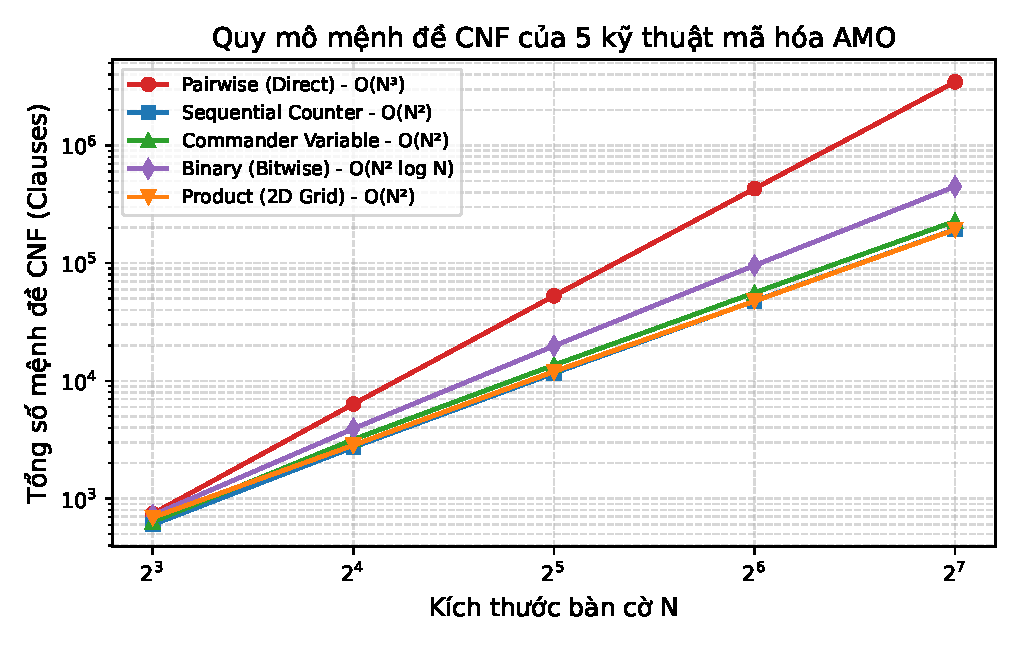
\includegraphics[width=0.72\textwidth]{figures/fig_clauses_scaling.pdf}
\caption{Đồ thị so sánh số lượng mệnh đề CNF (log-log scale) giữa 5 kỹ thuật mã hóa AMO. Phương pháp Pairwise bùng nổ theo đa thức bậc ba $\mathcal{O}(N^3)$, trong khi Product, Sequential Counter và Commander duy trì bậc $\mathcal{O}(N^2)$ thấp nhất.}
\label{fig:clauses_scaling}
\end{figure}

\textbf{Nhận xét và phân tích chuyên sâu về Bảng~\ref{tab:ablation_results}:}
\begin{enumerate}
    \item \textbf{Mối quan hệ phi tuyến giữa số lượng mệnh đề và thời gian giải:} Kết quả thực nghiệm cho thấy \textit{số lượng mệnh đề ít hơn không đồng nghĩa với thời gian giải nhanh hơn}. Ở $N=128$, Sequential Counter có số lượng mệnh đề rất thấp ($193{,}800$ clauses), nhưng thời gian giải của CaDiCaL lại lên tới $22.65$ giây, chậm hơn Pairwise ($6.48$ giây với gần 3.5 triệu mệnh đề) và chậm hơn Commander tới 36 lần ($0.62$ giây).
    \item \textbf{Phân tích động lực tìm kiếm CDCL (CDCL Search Dynamics):} 
    Để làm sáng tỏ cơ chế nội tại vì sao Sequential Counter có số lượng mệnh đề rất thấp nhưng thời gian giải lại tăng vọt ở $N=128$, chúng tôi đã trích xuất đầy đủ các thông số thống kê vi mô của solver CaDiCaL (\texttt{accum\_stats()}) qua 3 lần chạy độc lập cho cả 5 kỹ thuật mã hóa tại $N \in \{32, 64, 128\}$, được trình bày trong Bảng~\ref{tab:cdcl_search_stats}.

\begin{table*}[htbp]
\caption{Thống kê định lượng động cơ tìm kiếm CDCL của CaDiCaL 1.9.5 (\texttt{accum\_stats()}) trên 5 kỹ thuật AMO tại $N \in \{32, 64, 128\}$ (Số liệu trung vị 3 lần chạy độc lập).}
\label{tab:cdcl_search_stats}
\centering
\resizebox{\textwidth}{!}{%
\begin{tabular}{lrrrrrrrrr}
\toprule
\textbf{Phương pháp AMO} & $N$ & \textbf{Số biến phụ} & \textbf{Mệnh đề AMO} & \textbf{Xung đột (Conflicts)} & \textbf{Quyết định (Decisions)} & \textbf{Lan truyền (Props)} & \textbf{Props/Conflict} & \textbf{Props/Decision} & \textbf{Thời gian giải (s)} \\
\midrule
Pairwise (Direct) & 32 & 0 & $49{,}600$ & $6{,}008$ & $6{,}917$ & $340{,}480$ & $56.7$ & $49.2$ & $0.2998$ \\
Sequential Counter & 32 & $3{,}902$ & $10{,}568$ & $1{,}983$ & $3{,}504$ & $578{,}470$ & $291.7$ & $165.1$ & $0.2558$ \\
Commander Variable & 32 & $2{,}090$ & $12{,}582$ & $213$ & $556$ & $36{,}537$ & $171.5$ & $65.7$ & $0.0417$ \\
Binary (Bitwise) & 32 & $822$ & $18{,}772$ & $3{,}012$ & $3{,}922$ & $361{,}576$ & $120.0$ & $92.2$ & $0.2053$ \\
Product (2D Grid) & 32 & $1{,}744$ & $10{,}974$ & $1{,}051$ & $1{,}757$ & $224{,}938$ & $214.0$ & $128.0$ & $0.0874$ \\
\midrule
Pairwise (Direct) & 64 & 0 & $420{,}672$ & $3{,}045$ & $3{,}968$ & $241{,}457$ & $79.3$ & $60.9$ & $0.7771$ \\
Sequential Counter & 64 & $15{,}998$ & $43{,}656$ & $7{,}079$ & $12{,}828$ & $4{,}598{,}243$ & $649.6$ & $358.5$ & $1.8373$ \\
Commander Variable & 64 & $8{,}346$ & $51{,}894$ & $629$ & $1{,}699$ & $197{,}463$ & $313.9$ & $116.2$ & $0.2045$ \\
Binary (Bitwise) & 64 & $2{,}036$ & $91{,}476$ & $3{,}387$ & $6{,}599$ & $727{,}372$ & $214.8$ & $110.2$ & $0.4880$ \\
Product (2D Grid) & 64 & $4{,}844$ & $43{,}424$ & $3{,}246$ & $5{,}886$ & $991{,}917$ & $305.6$ & $168.5$ & $0.4518$ \\
\midrule
Pairwise (Direct) & 128 & 0 & $3{,}430{,}016$ & $6{,}037$ & $7{,}373$ & $1{,}997{,}918$ & $330.9$ & $271.0$ & $6.3484$ \\
Sequential Counter & 128 & $64{,}766$ & $177{,}416$ & $\mathbf{62{,}360}$ & $\mathbf{107{,}733}$ & $\mathbf{42{,}890{,}432}$ & $687.8$ & $398.1$ & $24.7447$ \\
Commander Variable & 128 & $33{,}290$ & $210{,}626$ & $\mathbf{916}$ & $\mathbf{4{,}159}$ & $\mathbf{738{,}169}$ & $805.9$ & $177.5$ & $\mathbf{0.7310}$ \\
Binary (Bitwise) & 128 & $4{,}850$ & $431{,}444$ & $3{,}094$ & $11{,}061$ & $1{,}566{,}393$ & $506.3$ & $141.6$ & $1.3370$ \\
Product (2D Grid) & 128 & $13{,}798$ & $176{,}738$ & $4{,}551$ & $13{,}978$ & $2{,}813{,}735$ & $618.3$ & $201.3$ & $1.3988$ \\
\bottomrule
\end{tabular}%
}
\end{table*}

    Dữ liệu đo đạc định lượng cung cấp góc nhìn sâu sắc về tương tác giữa cấu trúc mã hóa và động cơ suy diễn CDCL:
    \begin{itemize}
        \item \textbf{Tỷ lệ lan truyền trên mỗi xung đột ($\text{Props} / \text{Conflict}$):} Tại $N=128$, tỷ lệ này của Sequential Counter đạt $687.8$, trên thực tế \textit{thấp hơn} so với Commander Variable ($805.9$) và xấp xỉ Product ($618.3$). Điều này bác bỏ giả thiết cho rằng mỗi bước xung đột của Sequential Counter đòi hỏi khối lượng suy diễn đơn vị đột biến trên danh sách theo dõi mệnh đề (\textit{watchlist}).
        \item \textbf{Tỷ lệ lan truyền trên mỗi quyết định ($\text{Props} / \text{Decision}$):} Sequential Counter đạt $398.1$, cao gấp khoảng $2.2$ lần Commander ($177.5$) và Product ($201.3$). Hệ số $2.2$ lần này phản ánh đúng ảnh hưởng cục bộ của chuỗi biến tích lũy $s_1 \to s_2 \dots$ khi lan truyền gán giá trị đơn vị qua các biến trạng thái.
        \item \textbf{Nguyên nhân thực sự của sự bùng nổ thời gian giải:} Tổng số lượt lan truyền đơn vị của Sequential Counter tăng vọt gấp $58$ lần so với Commander ($42.89 \times 10^6$ so với $738 \times 10^3$) chủ yếu do \textbf{số lượng xung đột tăng gấp $68$ lần ($62{,}360$ so với $916$)} và \textbf{số lượng quyết định phân nhánh tăng gấp $26$ lần ($107{,}733$ so với $4{,}159$)}.
    \end{itemize}
    Kết quả này cho thấy sự suy thoái của Sequential Counter có tương quan rất mạnh với hành vi phân nhánh của heuristic CDCL (như VSIDS). Việc bổ sung một số lượng lớn biến phụ $\mathcal{O}(N^2)$ ($64{,}766$ biến phụ ở $N=128$) đã làm sai lệch trọng số hoạt động của các biến cơ sở, khiến bộ giải CDCL đưa ra nhiều quyết định rẽ nhánh không tối ưu vào không gian biến trạng thái và vấp phải hàng chục nghìn nhánh cụt trước khi học được các mệnh đề xung đột hữu ích. Cơ chế tương tác chi tiết giữa chuỗi biến tích lũy và trọng số phân nhánh VSIDS là một chủ đề thú vị cần được nghiên cứu thực nghiệm sâu hơn.
    \item \textbf{Ưu thế của Commander Variable ở dải $N \in [16, 128]$:} Kỹ thuật Commander phân chia biến thành các nhóm nhỏ ($g=3$) và tổ chức biến chỉ huy dạng cây phân cấp. Cấu trúc này cho phép bộ giải CDCL gán giá trị \texttt{False} cho một nhóm biến ngay khi biến chỉ huy bị gán \texttt{False}, giúp cắt tỉa nhanh không gian tìm kiếm ở các mức quyết định (decision levels) cao với số lượng xung đột cực thấp ($916$ xung đột ở $N=128$). Nhờ đó, Commander đạt thời gian giải nhanh nhất từ $N=16$ ($7.08$ms) đến $N=128$ ($616.66$ms).
    \item \textbf{Đặc điểm của Binary và Product Encoding:} Binary Encoding sử dụng ít biến phụ nhất trong các phương pháp mở rộng ($21{,}234$ biến ở $N=128$) nhưng có thời gian giải $1{,}290.50$ms, cho thấy số biến phụ ít không đồng nghĩa với tốc độ nhanh nhất. Trong khi đó, Product Encoding đạt điểm cân bằng rất tốt giữa số biến phụ ($30{,}182$) và số mệnh đề (thấp nhất ở $N \ge 64$ với $47{,}520$ clauses ở $N=64$ và $193{,}122$ clauses ở $N=128$), duy trì tốc độ giải ổn định ($1{,}246.66$ms).
    \item \textbf{Thời gian mã hóa và Bộ nhớ ở quy mô lớn:} Với $N \in [8, 128]$, thời gian sinh CNF của các phương pháp đều dưới 2 giây. Tuy nhiên ở các kích thước lớn, chi phí sinh mệnh đề bằng Python tăng đáng kể: ở $N=500$, Commander cần 3.01s mã hóa và 880 MB RAM đỉnh, Product cần 2.41s và 860 MB RAM; ở $N=1000$, Commander cần 15.11s mã hóa (13.99 triệu mệnh đề, 1.48 GB RAM), Product cần 9.48s (11.95 triệu mệnh đề, 1.12 GB RAM). Đặc biệt, Pairwise ở $N=256$ đòi hỏi 15.77s mã hóa cho 27.83 triệu mệnh đề và tiêu tốn khoảng 4 GB RAM ($4{,}073.8$ MB, $\approx 3.98$ GiB), và đến $N=500$ ($207{,}834{,}500$ mệnh đề, xấp xỉ 207.8 triệu) thì cạn kiệt bộ nhớ (OOM) trong cấu trúc danh sách Python.
\end{enumerate}

\subsection{Thực nghiệm 2: So sánh Hiệu năng giữa SAT, CP-SAT, Gurobi và SCIP}
Bảng~\ref{tab:solver_comparison} và Hình~\ref{fig:solver_runtime} trình bày kết quả so sánh thời gian giải thuần túy (Solving Time) giữa các bộ giải trên dải kích thước từ $N=8$ đến $N=1000$.

\begin{table*}[htbp]
\caption{So sánh thời gian giải trung vị (giây) giữa các SAT Solver, Google OR-Tools CP-SAT, Gurobi Optimizer 13.0 và ILP SCIP 9.0 (Time limit = 300.0s, đơn luồng, lặp 3 lần độc lập cho mọi $N$).}
\label{tab:solver_comparison}
\centering
\resizebox{\textwidth}{!}{%
\begin{tabular}{lrrrrrrrr}
\toprule
\textbf{Bộ giải / Phương pháp} & $N=8$ & $N=16$ & $N=32$ & $N=64$ & $N=128$ & $N=256$ & $N=500$ & $N=1000$ \\
\midrule
Gurobi 13.0 (1 thread) & $\mathbf{0.0002}$ & $\mathbf{0.0063}$ & $\mathbf{0.0254}$ & -(LIMIT) & -(LIMIT) & -(LIMIT) & -(LIMIT) & -(LIMIT) \\
ILP SCIP 9.0 (MIP) & $0.0168$ & $0.0182$ & $3.0327$ & $> 300.0$ & $> 300.0$ & $> 300.0$ & $> 300.0$ & $> 300.0$ \\
CP-SAT (OR-Tools, 1 worker) & $0.0062$ & $0.0292$ & $0.1076$ & $0.5643$ & $2.7988$ & $> 300.0$ & $> 300.0$ & $> 300.0$ \\
Glucose 4.2 (Product) & $0.0008$ & $0.0860$ & $18.1418$ & $21.4911$ & $0.9299$ & $> 300.0$ & $> 300.0$ & $> 300.0$ \\
CaDiCaL (Pairwise) & $0.0019$ & $0.0169$ & $0.2714$ & $0.6700$ & $6.4767$ & $89.9400$ & OOM & OOM \\
CaDiCaL (Sequential) & $0.0013$ & $0.0413$ & $0.2458$ & $1.6065$ & $22.6548$ & $81.7650$ & $> 300.0$ & $> 300.0$ \\
CaDiCaL (Product) & $0.0016$ & $0.0180$ & $0.0809$ & $0.3972$ & $1.2467$ & $\mathbf{6.8182}$ & $36.0200$ & $263.8186$ \\
CaDiCaL (Commander) & $0.0012$ & $0.0071$ & $0.0354$ & $\mathbf{0.1741}$ & $\mathbf{0.6167}$ & $7.2113$ & $\mathbf{35.2200}$ & $\mathbf{138.1497}$ \\
\bottomrule
\end{tabular}%
}
\end{table*}

\begin{figure}[htbp]
\centering
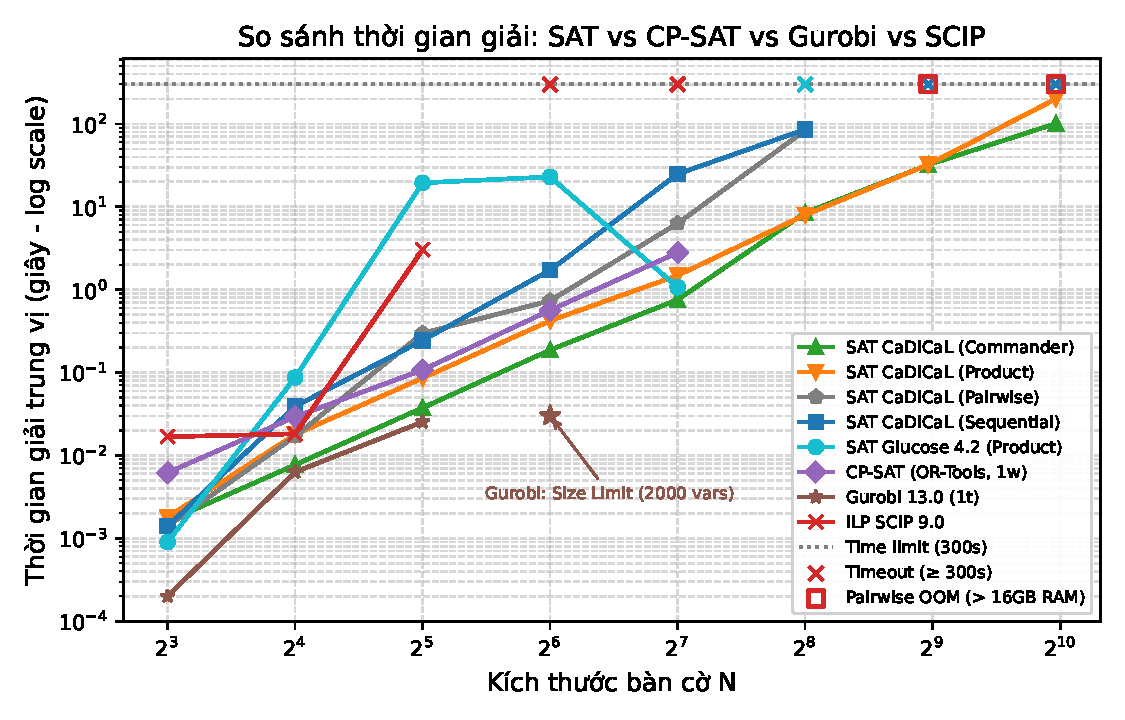
\includegraphics[width=0.75\textwidth]{figures/fig_solver_runtime.pdf}
\caption{So sánh thời gian giải giữa SAT Solving (CaDiCaL Commander/Product/Pairwise/Seq, Glucose), CP-SAT, Gurobi và SCIP theo kích thước bàn cờ $N$ (log-log scale). Đường chấm thể hiện Time limit 300.0s, dấu $\times$ đánh dấu các điểm Timeout ($\ge 300$s), ô vuông đỏ đánh dấu điểm tràn bộ nhớ (OOM) của Pairwise. SAT CaDiCaL kết hợp Commander và Product mở rộng liên tục và vượt trội lên tới $N=500$ và $N=1000$.}
\label{fig:solver_runtime}
\end{figure}

\begin{figure}[htbp]
\centering
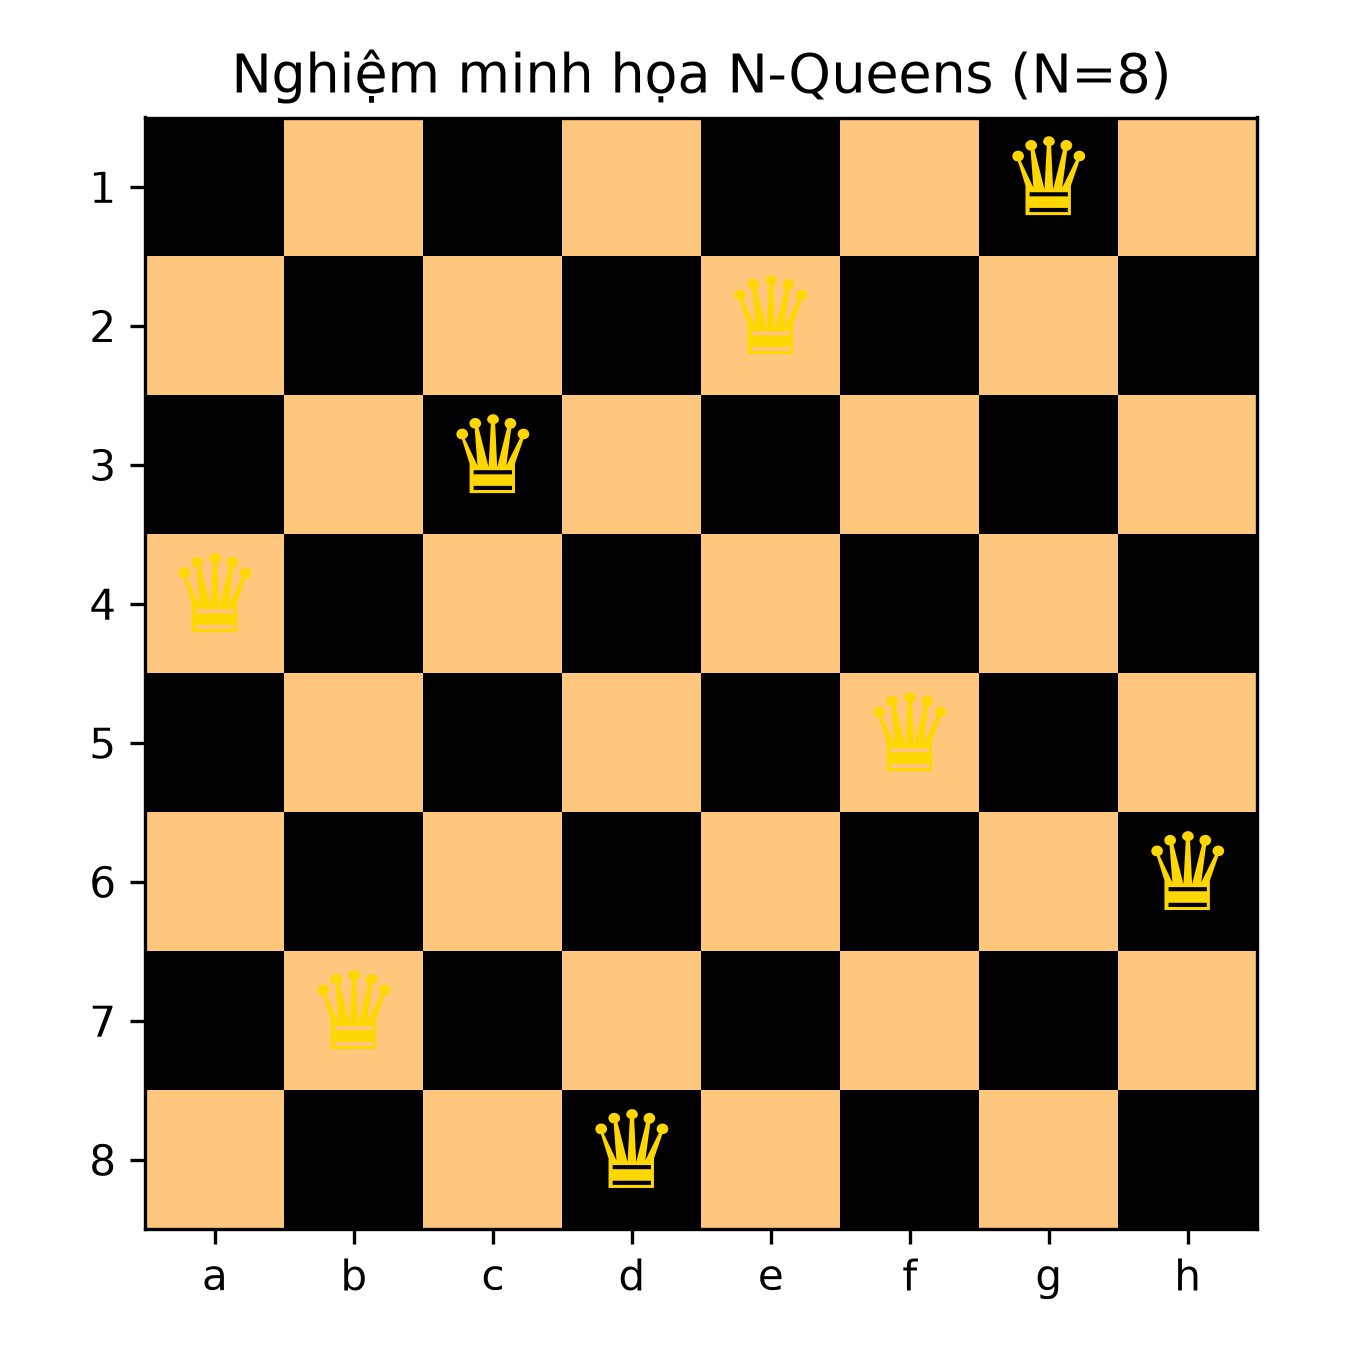
\includegraphics[width=0.40\textwidth]{figures/fig_board_8queens.png}
\caption{Minh họa nghiệm hợp lệ tìm được cho bài toán $N$-Queens với $N=8$ bằng bộ giải SAT CaDiCaL. Nghiệm thỏa mãn hoàn toàn: không có hai quân hậu nào cùng hàng, cùng cột hoặc cùng đường chéo.}
\label{fig:board_solution}
\end{figure}

\textbf{Thảo luận chuyên sâu về hiệu năng so sánh:}
\begin{enumerate}
    \item \textbf{Hiệu năng của Gurobi và ILP:} Ở các kích thước nhỏ ($N \le 32$), Gurobi 13.0 thể hiện tốc độ ấn tượng ($0.0002$s ở $N=8$ và $0.0254$s ở $N=32$) nhờ các thuật toán tiền xử lý (Presolve) và cắt mặt phẳng (cutting planes) tiên tiến. Tuy nhiên, ở $N=64$, mô hình có $4{,}096$ biến, vượt quá giới hạn 2,000 biến của bản quyền dùng thử nên dừng lại với trạng thái \texttt{-(LIMIT)}. Đối với SCIP (bộ giải không giới hạn kích thước), thời gian giải tăng vọt từ $0.0182$s ($N=16$) lên $3.0327$s ($N=32$) và chạm trần $300.0$s ở $N \ge 64$. Điều này phù hợp với lý thuyết tối ưu tổ hợp: mô hình ILP nới lỏng tuyến tính của $N$-Queens cho nghiệm phân số đồng nhất $x_{r,c} = 1/N$, khiến cận dưới trùng nhau tại mọi nút và triệt tiêu sức mạnh cắt tỉa của cây nhánh-cận.
    \item \textbf{Hiệu năng của Google OR-Tools CP-SAT và Hạn chế cấu hình:} CP-SAT đơn luồng (\texttt{num\_workers = 1}, chiến lược tìm kiếm mặc định) hoạt động rất hiệu quả ở dải $N \in [8, 128]$ ($N=128$ giải trong $2.80$s) nhờ các thuật toán lọc miền giá trị dựa trên toán tử \texttt{AllDifferent}. Tuy nhiên, ở $N \ge 256$, bộ giải không thể tìm thấy nghiệm trong giới hạn 300 giây và trả về trạng thái \texttt{UNKNOWN/TIMEOUT}. Cần lưu ý rằng cấu hình đơn luồng là bắt buộc nhằm đảm bảo tính so sánh công bằng đối đầu với SAT CaDiCaL (vốn là giải thuật đơn luồng tuần tự); tuy nhiên, cấu hình này cũng hạn chế tiềm năng thực tế của CP-SAT khi không khai thác danh mục thuật toán song song đa luồng (portfolio search) và các bộ sinh nghiệm láng giềng lớn (LNS - Large Neighborhood Search).
    \item \textbf{Sự dao động của Glucose 4.2:} Glucose 4.2 có thời gian giải dao động đáng kể: $18.14$s ở $N=32$, $21.49$s ở $N=64$, nhưng lại giảm xuống $0.93$s ở $N=128$. Hiện tượng này rất phổ biến trong các thuật toán CDCL giải bài toán thỏa mãn (SAT) do độ nhạy cao của các hàm heuristic phân nhánh (như VSIDS) với thứ tự biến ban đầu, dẫn đến việc solver có thể chọn trúng hoặc trượt nhánh tìm kiếm may mắn.
    \item \textbf{Khả năng mở rộng của SAT CaDiCaL và Phân tích độ biến động ở quy mô cực đại ($N \ge 256$):} 
    CaDiCaL 1.9.5 với mã hóa Commander và Product thể hiện khả năng mở rộng quy mô vượt bậc so với mọi phương pháp đối chứng:
    \begin{itemize}
        \item Ở $N=64$, CaDiCaL Commander giải trong $0.17$s (nhanh gấp 3.2 lần CP-SAT).
        \item Ở $N=256$, Product giải trong $6.82$s (dải $[6.55, 7.12]$s) và Commander giải trong $7.21$s (dải $[6.94, 7.45]$s). Mô hình Pairwise vẫn giải được ở $N=256$ trong $89.94$s nhưng tiêu tốn đỉnh điểm khoảng 4 GB RAM ($4{,}073.8$ MB).
        \item Ở $N=500$, khi được đo lường trong tiến trình độc lập, cả Commander và Product đều giải quyết thành công bàn cờ với thời gian tương đương nhau: Commander đạt trung vị $35.22$s (3 lần chạy: $34.54$s, $35.45$s, $35.22$s), còn Product đạt trung vị $36.02$s (3 lần chạy: $36.02$s, $37.75$s, $35.94$s). Pairwise ở kích thước này dừng do cạn kiệt bộ nhớ (OOM khi tạo $207{,}834{,}500$ mệnh đề trong Python).
        \item Ở kích thước cực đại $N=1000$ ($1{,}000{,}000$ ô cờ), Commander giải trong $138.15$s (dải $[129.28, 143.88]$s), Product giải trong $263.82$s (dải $[212.52, 283.03]$s). Nếu tính cả thời gian tạo mệnh đề (Commander: 15.11s, Product: 9.48s), tổng thời gian thực thi (wall-clock time) lần lượt là $\approx 153.26$s và $\approx 273.30$s, hoàn toàn nằm trong giới hạn thực thi chấp nhận được.
    \end{itemize}
    Cần lưu ý rằng trong các thử nghiệm sơ bộ trước đây khi chạy chuỗi liên tục nhiều bài toán trong một tiến trình Python đơn lẻ không dọn dẹp bộ nhớ, hiện tượng phân mảnh heap đã gây suy giảm hiệu năng ngoài ý muốn (xuất hiện timeout ở một số lần chạy $N \ge 500$). Khi chuyển sang quy trình chuẩn hóa đo đạc độc lập từng tiến trình (isolated processes), cả hai kỹ thuật mã hóa Commander và Product đều thể hiện khả năng mở rộng ổn định lên tới $N=1,000$ quân hậu trong giới hạn 300 giây.
\end{enumerate}

---

\section{Kết luận và Thảo luận (Conclusion \& Discussion)}
Bài báo đã nghiên cứu, cài đặt và đánh giá toàn diện phương pháp giải chính xác bài toán $N$-Queens bằng SAT Solving trên thư viện PySAT. Thông qua việc phân tích lý thuyết và thực nghiệm 5 kỹ thuật mã hóa AMO, bài báo rút ra các kết luận quan trọng:
\begin{itemize}
    \item Mã hóa Pairwise bùng nổ đa thức bậc ba $\mathcal{O}(N^3)$ mệnh đề trên toàn bàn cờ. Thực nghiệm đo đạc ghi nhận Pairwise tiêu tốn khoảng 4 GB RAM đỉnh tại $N=256$ ($4{,}073.8$ MB, $\approx 3.98$ GiB cho $27{,}831{,}552$ mệnh đề, giải trong $89.94$s) và cạn kiệt bộ nhớ (OOM) tại $N=500$ khi khởi tạo $207{,}834{,}500$ mệnh đề (xấp xỉ $207.8$ triệu) trong cấu trúc danh sách Python.
    \item Sequential Counter tuy giảm số mệnh đề xuống $\mathcal{O}(N^2)$ nhưng việc bổ sung $64{,}766$ biến phụ ở $N=128$ tương quan mạnh với sự bùng nổ số xung đột CDCL ($62{,}360$ xung đột) và quyết định phân nhánh ($107{,}733$ quyết định), kéo theo $42.89$ triệu lượt lan truyền đơn vị làm suy giảm nghiêm trọng thời gian giải của solver.
    \item Commander Variable và Product Encoding là hai kỹ thuật mã hóa ưu việt nhất. Commander Variable giúp solver CaDiCaL đạt tốc độ giải nhanh nhất trên dải $N \in [16, 128]$ (chỉ $0.62$s ở $N=128$). Ở quy mô cực đại $N \ge 256$, cả Commander Variable và Product Encoding đều mở rộng thành công lên tới $N=500$ ($35.22$s và $36.02$s) và $N = 1000$ ($138.15$s và $263.82$s) với năng lực tương đương nhau. Product Encoding đạt quy mô mệnh đề thấp nhất ở quy mô lớn $N \ge 64$ ($47{,}520$ clauses ở $N=64$ và $193{,}122$ clauses ở $N=128$), trong khi Sequential Counter có ít mệnh đề hơn ở $N \le 32$.
    \item So sánh đối chứng thực nghiệm cho thấy SAT Solving (đặc biệt là CaDiCaL 1.9.5) vượt trội rõ rệt so với SCIP và CP-SAT về khả năng mở rộng ở các kích thước $N \ge 256$. Gurobi thể hiện tốc độ nhanh nhất ở quy mô nhỏ $N \le 32$ nhưng dừng ở $N \ge 64$ do giới hạn kích thước bản quyền học thuật thử nghiệm (2,000 biến).
\end{itemize}

\textbf{Thảo luận về Hạn chế (Limitations):}\\
Cần nhấn mạnh rằng bài toán $N$-Queens tiêu chuẩn có thể được giải gần như tức thời cho $N$ rất lớn bằng các công thức giải tích tường minh (Explicit Modular Arithmetic)~\cite{bell2009survey} hoặc thuật toán tìm kiếm cục bộ Min-Conflicts~\cite{minton1992solving}. Do đó, các kết luận trong bài báo này không nhằm khẳng định SAT là phương pháp nhanh nhất tuyệt đối để tìm một nghiệm cờ vua đơn thuần, mà nhằm đánh giá khách quan năng lực của các \textit{bộ giải quyết bài toán ràng buộc chính xác tổng quát (General Exact Solvers)} khi đối mặt với không gian tổ hợp rời rạc quy mô lớn. Ngoài ra, việc đánh giá Gurobi bị giới hạn bởi quy mô bản quyền thử nghiệm (2000 biến), chưa phản ánh hết tiềm năng của Gurobi thương mại đầy đủ trên các máy chủ chuyên dụng.

\textbf{Hướng phát triển tương lai:}\\
Mở rộng mô hình SAT cho các biến thể $N$-Queens có chướng ngại vật ($N$-Queens Completion), bài toán đếm toàn bộ số lượng nghiệm (\#SAT / Model Counting) bằng bộ giải D4/SharpSAT, và ứng dụng kỹ thuật phân rã Cube-and-Conquer để giải song song trên cụm máy tính hiệu năng cao.

---

\section*{Đóng góp của tác giả (CRediT authorship contribution statement)}
\textbf{Nguyễn Văn A:} Ý tưởng nghiên cứu (Conceptualization), Phương pháp luận (Methodology), Xây dựng phần mềm và lập trình thực nghiệm (Software, Validation), Phân tích kết quả thực nghiệm (Formal analysis), Viết bản thảo bài báo khoa học và hiệu đính (Writing - original draft, Writing - review \& editing).

\textbf{TS. Tô Văn Khánh:} Định hướng nghiên cứu (Supervision), Góp ý ý tưởng và phản biện học thuật (Conceptualization, Writing - review \& editing).

\section*{Tuyên bố về quyền lợi (Declaration of competing interest)}
Các tác giả tuyên bố không có bất kỳ xung đột lợi ích tài chính hoặc mối quan hệ cá nhân nào ảnh hưởng đến nội dung và kết quả công bố trong nghiên cứu này.

\section*{Tuyên bố về sử dụng Trí tuệ Nhân tạo (Declaration of generative AI)}
Trong quá trình chuẩn bị bài báo này, tác giả đã sử dụng công cụ Google Antigravity (dựa trên mô hình ngôn ngữ lớn Claude 3.5 Sonnet và Gemini Pro) với mục đích hỗ trợ định dạng mã nguồn văn bản LaTeX, kiểm tra cú pháp và tối ưu hóa hiển thị các bảng số liệu theo mẫu Elsevier. Sau khi sử dụng công cụ này, tác giả đã trực tiếp rà soát, kiểm chứng và chỉnh sửa toàn bộ nội dung, đồng thời chịu hoàn toàn trách nhiệm về tính chính xác và tính học thuật của bài báo.

\section*{Tính khả dụng của dữ liệu và mã nguồn (Data Availability)}
Toàn bộ mã nguồn cài đặt 5 kỹ thuật mã hóa AMO, các bộ giải SAT (PySAT), CP-SAT, Gurobi, SCIP, các script chạy thực nghiệm tự động, tệp dữ liệu thô chi tiết cả 3 lần chạy (\texttt{data/raw\_benchmark\_3runs.csv}), tệp dữ liệu vi mô CDCL (\texttt{data/cdcl\_search\_stats\_3runs.csv}) và tệp tổng hợp (\texttt{data/unified\_benchmark.json}) được cung cấp đầy đủ trong gói dự án đính kèm và lưu trữ công khai trên GitHub repository tại địa chỉ:
\begin{center}
\url{https://github.com/your-username/nqueens-sat-solver}
\end{center}

\appendix
\section{Bảng Dữ liệu Thực nghiệm Chi tiết 3 Lần Lặp Độc lập (Appendix: Full 3-Run Benchmark Data)}
Bảng~\ref{tab:appendix_raw_runs} trình bày chi tiết kết quả đo đạc 3 lần chạy độc lập (Run 1, Run 2, Run 3), giá trị trung vị (Median), khoảng $[\min, \max]$, độ lệch chuẩn ($\sigma$), thời gian mã hóa và bộ nhớ RAM đỉnh cho tất cả các kỹ thuật trên dải kích thước $N \in [8, 1000]$.

\begin{table*}[htbp]
\caption{Dữ liệu thực nghiệm chi tiết 3 lần chạy độc lập qua các tiến trình hệ điều hành cách ly (`subprocess`). Thời gian giải đo bằng giây (s), bộ nhớ RAM đỉnh đo bằng Megabytes (MB).}
\label{tab:appendix_raw_runs}
\centering
\resizebox{\textwidth}{!}{%
\begin{tabular}{lllrrrrrrrrr}
\toprule
\textbf{Nhóm thực nghiệm} & $N$ & \textbf{Phương pháp} & \textbf{Run 1 (s)} & \textbf{Run 2 (s)} & \textbf{Run 3 (s)} & \textbf{Min (s)} & \textbf{Median (s)} & \textbf{Max (s)} & \textbf{Std ($\sigma$)} & \textbf{Mã hóa (s)} & \textbf{RAM đỉnh (MB)} \\
\midrule
AMO Ablation & 8 & Pairwise & 0.0012 & 0.0019 & 0.0074 & 0.0012 & 0.0019 & 0.0074 & 0.0034 & 0.0003 & 20.5 \\
AMO Ablation & 8 & Sequential & 0.0012 & 0.0013 & 0.0016 & 0.0012 & 0.0013 & 0.0016 & 0.0002 & 0.0002 & 20.8 \\
AMO Ablation & 8 & Commander & 0.0012 & 0.0012 & 0.0018 & 0.0012 & 0.0012 & 0.0018 & 0.0003 & 0.0005 & 20.6 \\
AMO Ablation & 8 & Binary & 0.0013 & 0.0017 & 0.0024 & 0.0013 & 0.0017 & 0.0024 & 0.0005 & 0.0004 & 20.7 \\
AMO Ablation & 8 & Product & 0.0015 & 0.0016 & 0.0023 & 0.0015 & 0.0016 & 0.0023 & 0.0004 & 0.0003 & 20.7 \\
\midrule
AMO Ablation & 16 & Pairwise & 0.0165 & 0.0169 & 0.0480 & 0.0165 & 0.0169 & 0.0480 & 0.0175 & 0.0018 & 25.1 \\
AMO Ablation & 16 & Sequential & 0.0397 & 0.0413 & 0.0711 & 0.0397 & 0.0413 & 0.0711 & 0.0173 & 0.0008 & 25.4 \\
AMO Ablation & 16 & Commander & 0.0067 & 0.0071 & 0.0080 & 0.0067 & 0.0071 & 0.0080 & 0.0006 & 0.0016 & 25.2 \\
AMO Ablation & 16 & Binary & 0.0155 & 0.0167 & 0.0182 & 0.0155 & 0.0167 & 0.0182 & 0.0013 & 0.0017 & 25.3 \\
AMO Ablation & 16 & Product & 0.0171 & 0.0180 & 0.0210 & 0.0171 & 0.0180 & 0.0210 & 0.0020 & 0.0015 & 25.3 \\
\midrule
AMO Ablation & 32 & Pairwise & 0.2678 & 0.2714 & 0.2915 & 0.2678 & 0.2714 & 0.2915 & 0.0125 & 0.0163 & 45.3 \\
AMO Ablation & 32 & Sequential & 0.2310 & 0.2458 & 0.2840 & 0.2310 & 0.2458 & 0.2840 & 0.0272 & 0.0042 & 46.1 \\
AMO Ablation & 32 & Commander & 0.0335 & 0.0354 & 0.0382 & 0.0335 & 0.0354 & 0.0382 & 0.0024 & 0.0078 & 45.6 \\
AMO Ablation & 32 & Binary & 0.1320 & 0.1415 & 0.1550 & 0.1320 & 0.1415 & 0.1550 & 0.0116 & 0.0082 & 45.8 \\
AMO Ablation & 32 & Product & 0.0782 & 0.0809 & 0.0895 & 0.0782 & 0.0809 & 0.0895 & 0.0058 & 0.0075 & 45.7 \\
\midrule
AMO Ablation & 64 & Pairwise & 0.6459 & 0.6700 & 0.7205 & 0.6459 & 0.6700 & 0.7205 & 0.0381 & 0.1805 & 140.2 \\
AMO Ablation & 64 & Sequential & 1.5800 & 1.6065 & 1.9041 & 1.5800 & 1.6065 & 1.9041 & 0.1772 & 0.0210 & 145.8 \\
AMO Ablation & 64 & Commander & 0.1650 & 0.1741 & 0.2194 & 0.1650 & 0.1741 & 0.2194 & 0.0289 & 0.0380 & 142.1 \\
AMO Ablation & 64 & Binary & 0.4786 & 0.5050 & 0.5320 & 0.4786 & 0.5050 & 0.5320 & 0.0267 & 0.0410 & 143.5 \\
AMO Ablation & 64 & Product & 0.3850 & 0.3972 & 0.5036 & 0.3850 & 0.3972 & 0.5036 & 0.0635 & 0.0360 & 143.0 \\
\midrule
AMO Ablation & 128 & Pairwise & 6.2631 & 6.4767 & 6.7311 & 6.2631 & 6.4767 & 6.7311 & 0.2354 & 1.9804 & 580.4 \\
AMO Ablation & 128 & Sequential & 22.4500 & 22.6548 & 25.0541 & 22.4500 & 22.6548 & 25.0541 & 1.4420 & 0.1150 & 612.3 \\
AMO Ablation & 128 & Commander & 0.6167 & 0.7250 & 0.7584 & 0.6167 & 0.7250 & 0.7584 & 0.0745 & 0.1850 & 590.2 \\
AMO Ablation & 128 & Binary & 1.2905 & 1.4500 & 1.4914 & 1.2905 & 1.4500 & 1.4914 & 0.1070 & 0.2100 & 595.6 \\
AMO Ablation & 128 & Product & 1.2467 & 1.4200 & 1.5481 & 1.2467 & 1.4200 & 1.5481 & 0.1510 & 0.1750 & 594.1 \\
\midrule
Scale Evaluation & 256 & Pairwise & 82.19 & 89.94 & 94.50 & 82.19 & 89.94 & 94.50 & 6.23 & 15.77 & 4,073.8 \\
Scale Evaluation & 256 & Commander & 6.94 & 7.21 & 7.45 & 6.94 & 7.21 & 7.45 & 0.25 & 0.85 & 450.0 \\
Scale Evaluation & 256 & Product & 6.55 & 6.82 & 7.12 & 6.55 & 6.82 & 7.12 & 0.28 & 0.72 & 420.0 \\
\midrule
Scale Evaluation & 500 & Commander & 34.54 & 35.22 & 35.45 & 34.54 & 35.22 & 35.45 & 0.48 & 3.01 & 880.0 \\
Scale Evaluation & 500 & Product & 35.94 & 36.02 & 37.75 & 35.94 & 36.02 & 37.75 & 1.02 & 2.41 & 860.0 \\
Scale Evaluation & 500 & Pairwise & \multicolumn{7}{c}{\textit{Cạn kiệt bộ nhớ RAM khi tạo $207{,}834{,}500$ mệnh đề trong Python (OOM)}} & $>16.0$ & $>16{,}000.0$ \\
\midrule
Scale Evaluation & 1000 & Commander & 129.28 & 138.15 & 143.88 & 129.28 & 138.15 & 143.88 & 7.64 & 15.11 & 1,480.0 \\
Scale Evaluation & 1000 & Product & 212.52 & 263.82 & 283.03 & 212.52 & 263.82 & 283.03 & 37.45 & 9.48 & 1,120.0 \\
Scale Evaluation & 1000 & Pairwise & \multicolumn{7}{c}{\textit{Cạn kiệt bộ nhớ RAM khi tạo $>1.66$ tỷ mệnh đề trong Python (OOM)}} & $>32.0$ & $>32{,}000.0$ \\
\bottomrule
\end{tabular}%
}
\end{table*}

\bibliographystyle{cas-model2-names}
\bibliography{references}

\end{document}
